\section{Development method}
We had very few requirements and technical restrictions when we received the project, which left the project open to interpretation. Therefore, we wanted to choose a flexible work methodology. Agile work methods focus on continuous planning throughout the process and having frequent communication with the client, in our case Accenture. We had meetings with our external supervisors from Accenture once every second week, which meant the agile model was a good fit for our project. We took inspiration from two light frameworks, Scrum and Kanban.

\subsection{Scrum and sprints}
Scrum is a framework that dictates how developers work in teams to solve complex problems. The development process is also divided into time intervals called a sprint. A sprint is an essential part of using the Scrum framework \parencite{prosjektveilederen}. Sprints are a fixed time length, often between one and four weeks. In this specified time length, the teams do tasks assigned from the sprint backlog. Each sprint starts with sprint planning and ends with a sprint retrospective.

We found it most viable for our project to plan in increments of two weeks. We chose two-week increments because we felt it was an even balance between work and planning. This time increment also fitted our bi-weekly meeting plan with our supervisors.

Our group also made use of the meetings in the Scrum framework. The meetings are sprint planning, sprint retrospective, and daily standups. Sprint planning is a meeting or event which starts before a sprint. During the sprint planning, the teams agree on a goal for the sprint and the tasks from the backlog that should be worked on that contribute to the goal. The backlog is a list of functionality the product should contain. In addition, we wrote down the tasks for the specific sprints in a digital document. These tasks were to be finished by the next sprint. \figref{fig:sprintoverview} is our sprint planning documents that show our goals for each sprint.

\begin{figure}[h!]
	\centering
	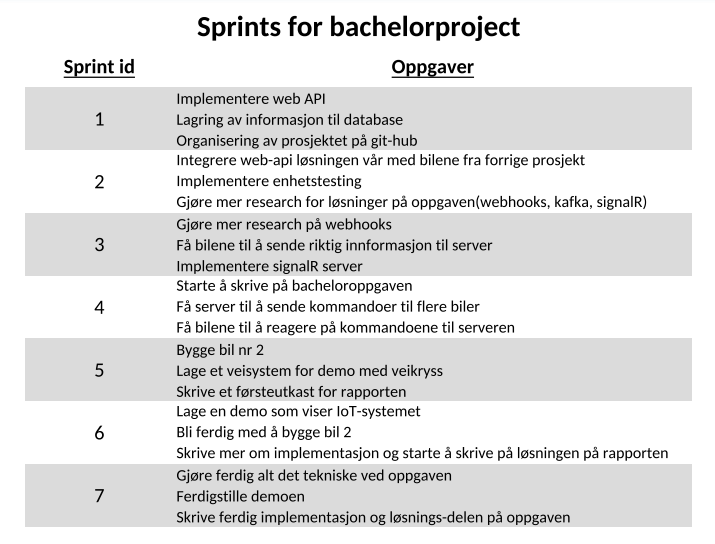
\includegraphics[width=1\linewidth]{figures/Sprint_overview}
	\caption[Sprint overview]{An overview of our sprints. Each sprint lasted 2 weeks.}
	\label{fig:sprintoverview}
\end{figure}

After a sprint, we would have a sprint retrospective to discuss what went well in that sprint and what could have been done better. We would also examine if the task assigned in the sprint meetings was finished or needed more work. These meetings helped us reflect over the prior week and adjust accordingly, if necessary. The sessions also helped us determine if we were on track with our initial plan. 
 
In addition to the weekly meetings, we also had daily standups. Daily standups are short meetings, usually lasting around five minutes, where each person answers three questions. What did the person do last time? What is the person going to do today? Are there any challenges? We implemented daily standups because it helped our team get on the same page, and it made it easier to plan what each of us had to do that specific day.

Scrum often consists of a team with different roles. As a team of three, we did not feel the necessity to have specified roles because we usually worked together on our projects. However, we alternated on being the scrum master. The scrum master's responsibility is to keep track of the backlog and lead the sprint planning meetings.

Our implementation of Kanban was to use a Kanban board as the backlog. We used a Kanban board to visualize where a task is in the work process. Here is an example from our project:

\begin{figure}[h!]
	\centering
	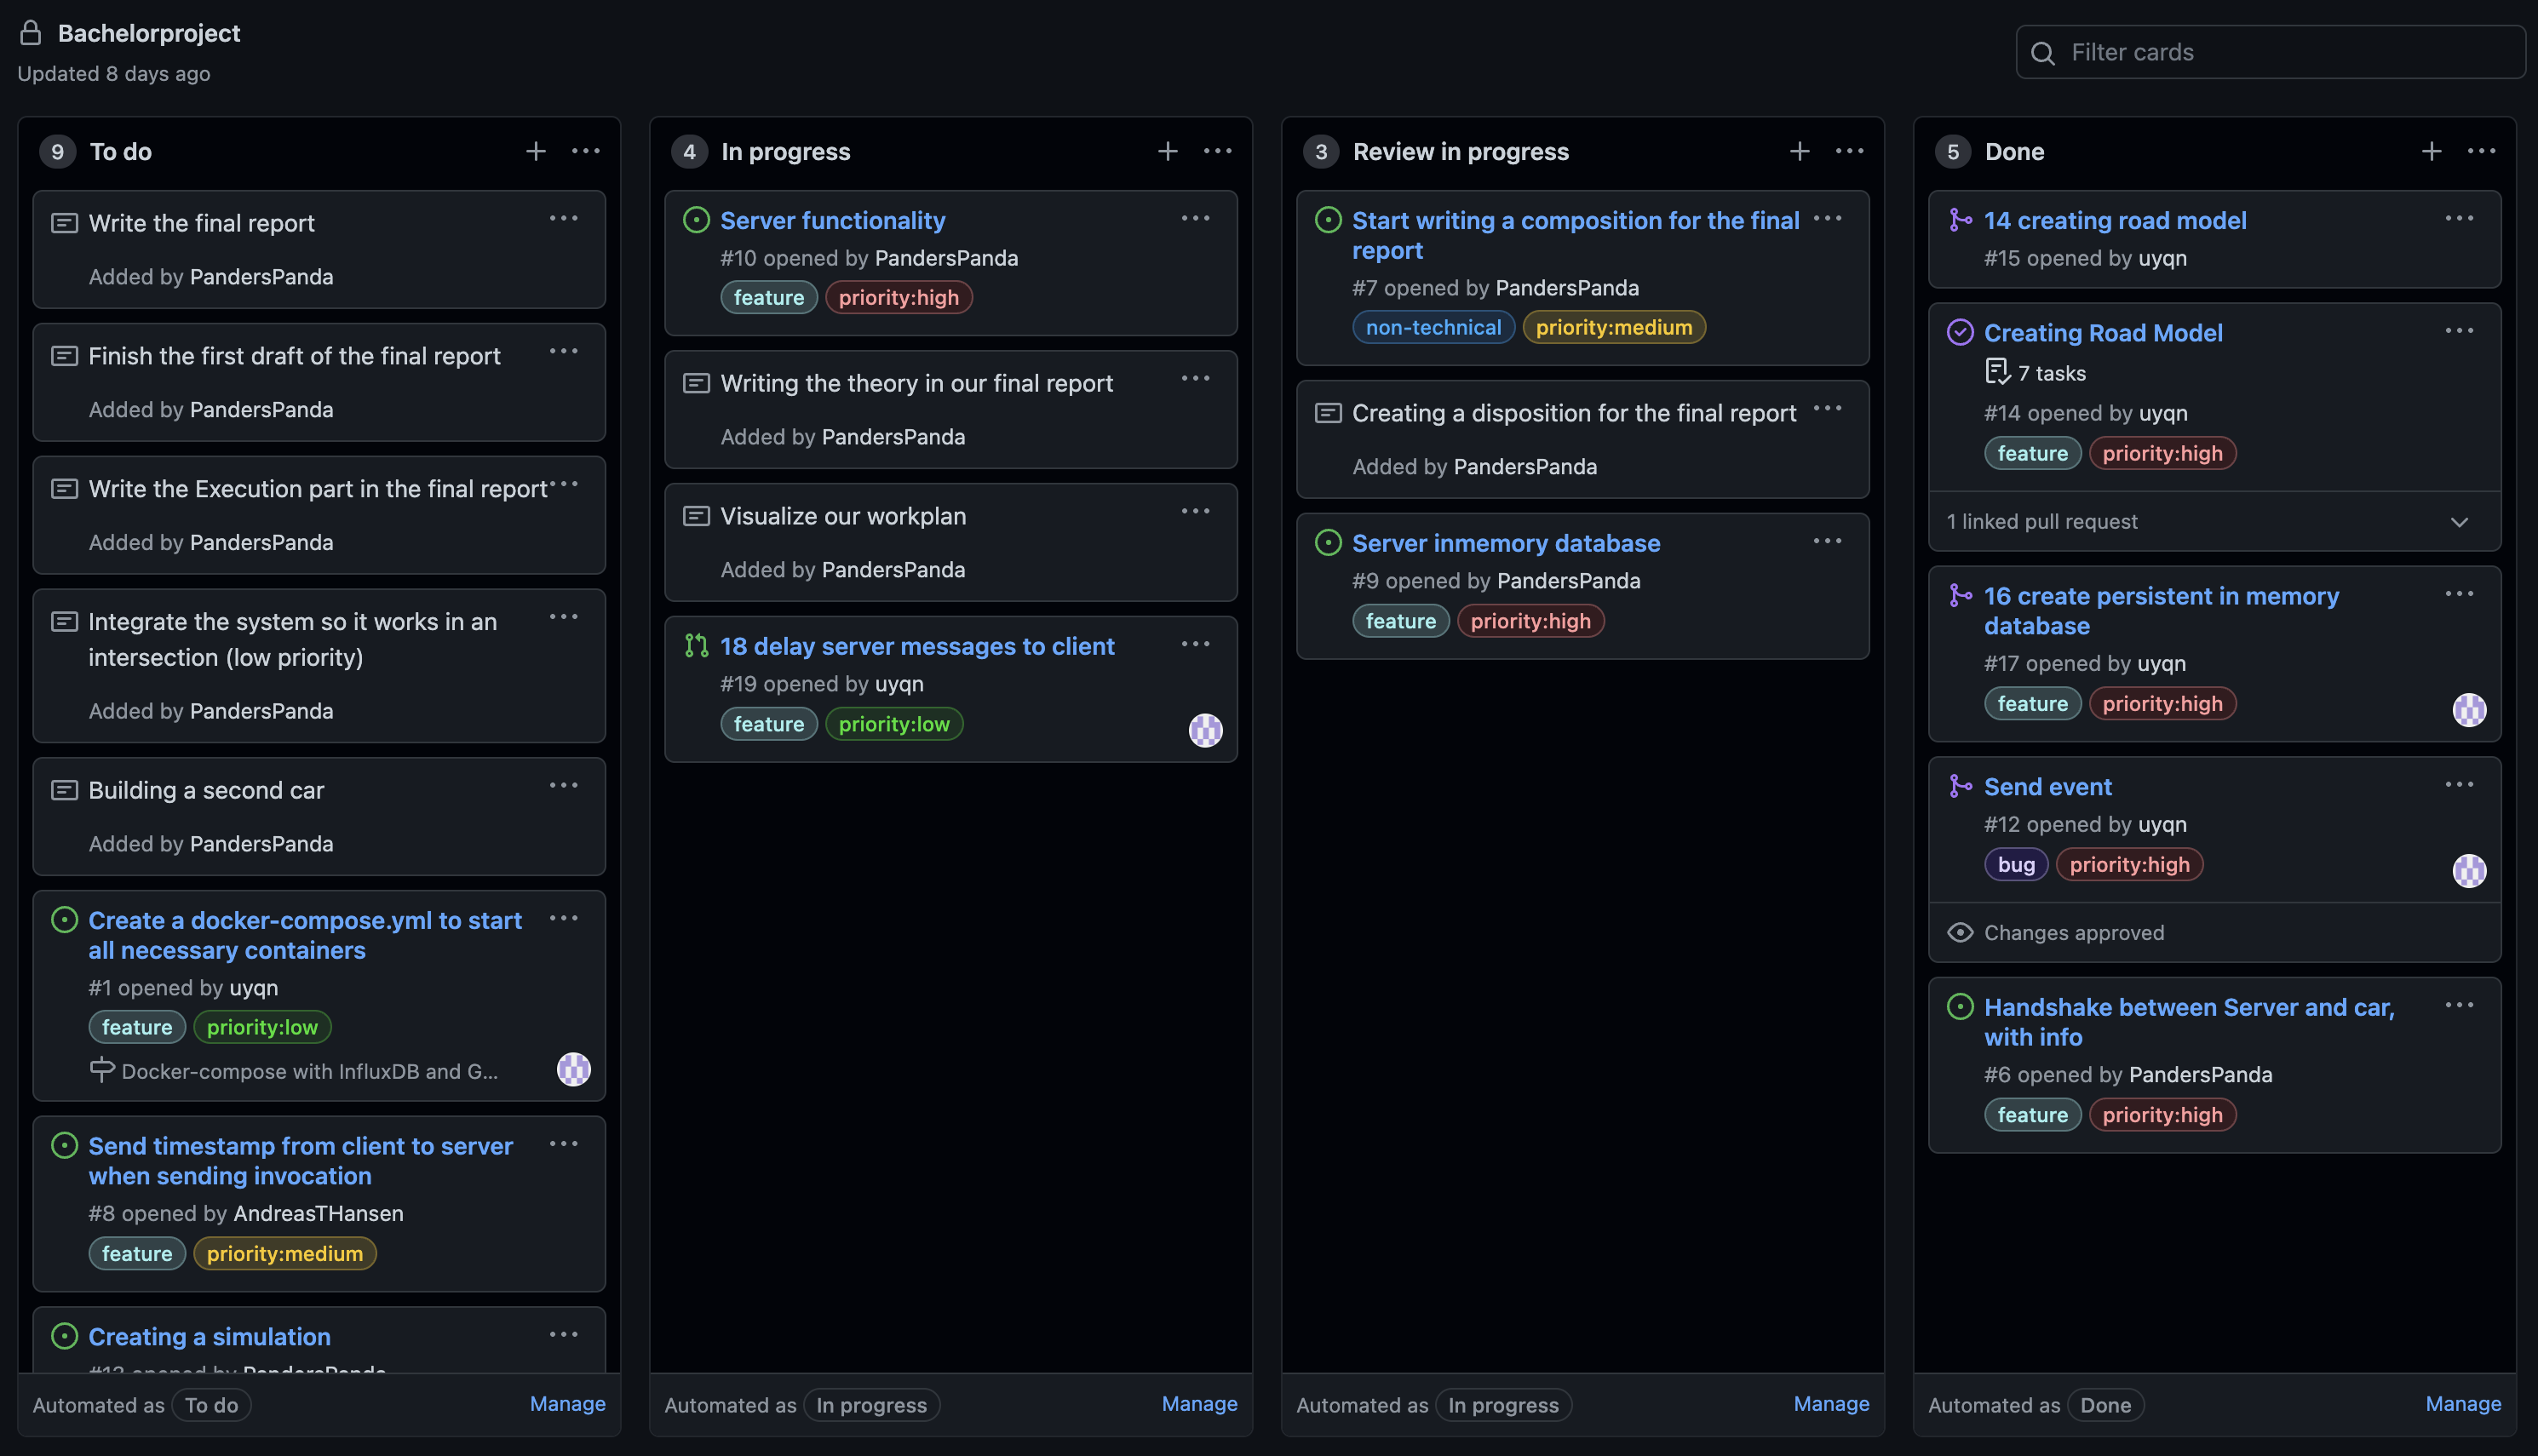
\includegraphics[width=1\linewidth]{figures/kanban_screenshot}
	\caption[kanban screenshot]{Extract of our kanban from Github.}
	\label{fig:kanbanscreenshot}
\end{figure}

We have four columns that represent which phase a task is in. The backlog is the tasks in the to-do column. We dragged it over to the "In progress"-column when we were working on a task. After finishing a task, it went to the "Review in progress"-column, where we reviewed it. If we concluded that the task was finished in the reviewing, it was dragged over to the "Done"-column. The git project tool also provides prioritization of tasks from high to low. We also took advantage of this. You can also connect the tasks to a specific branch, so the task automatically gets finished when merging the branch into the main branch. The Kanban board was a great tool to see which tasks to choose for our sprints and also keep track of where the tasks were in their process.

However, we did not use the Kanban board throughout the whole process. This is because the backlog was changing a lot, and the Kanban board needed many modifications to be up to date. We figured out that it was more beneficial to focus on one framework, which in our case was Scrum. In addition, we were able to keep track of the tasks by having frequent meetings. 